
\section{Dynarobin leg model}

This paper goal is to improove locomotion stability on quadrupedal robot Dynarobin, depicted in Fig. \ref{fig:Dynarobin}. Dynarobin has four identical legs ($i\in \left \{ 1,2,3,4 \right \}$), each combning three rotational joints: shoulder, elbow, and wrist, respectively. Additionally each leg containts mehanical spring which defines stiffnes to the contact surface. In order to obtain spring-mass compliante leg behavior, impedance or simillar torque based control can be used. The aproximative Dynarobin leg model is shown in \ref{fig:DynarobinLEG}. It consists of three masses connected by virtual active and passive spring. The passive spring has initial fixed length $L_{pi}=L_{p0}$ and parameters $K_{pi}$ and $C_{pi}$.  The actuated spring has variable parameters $K_{ai}$ and $C_{ai}$ and actuation is provided by changing the initial length $L_{ai}=L_{a0}$ by $\delta L$.
\begin{figure}
	\centering
	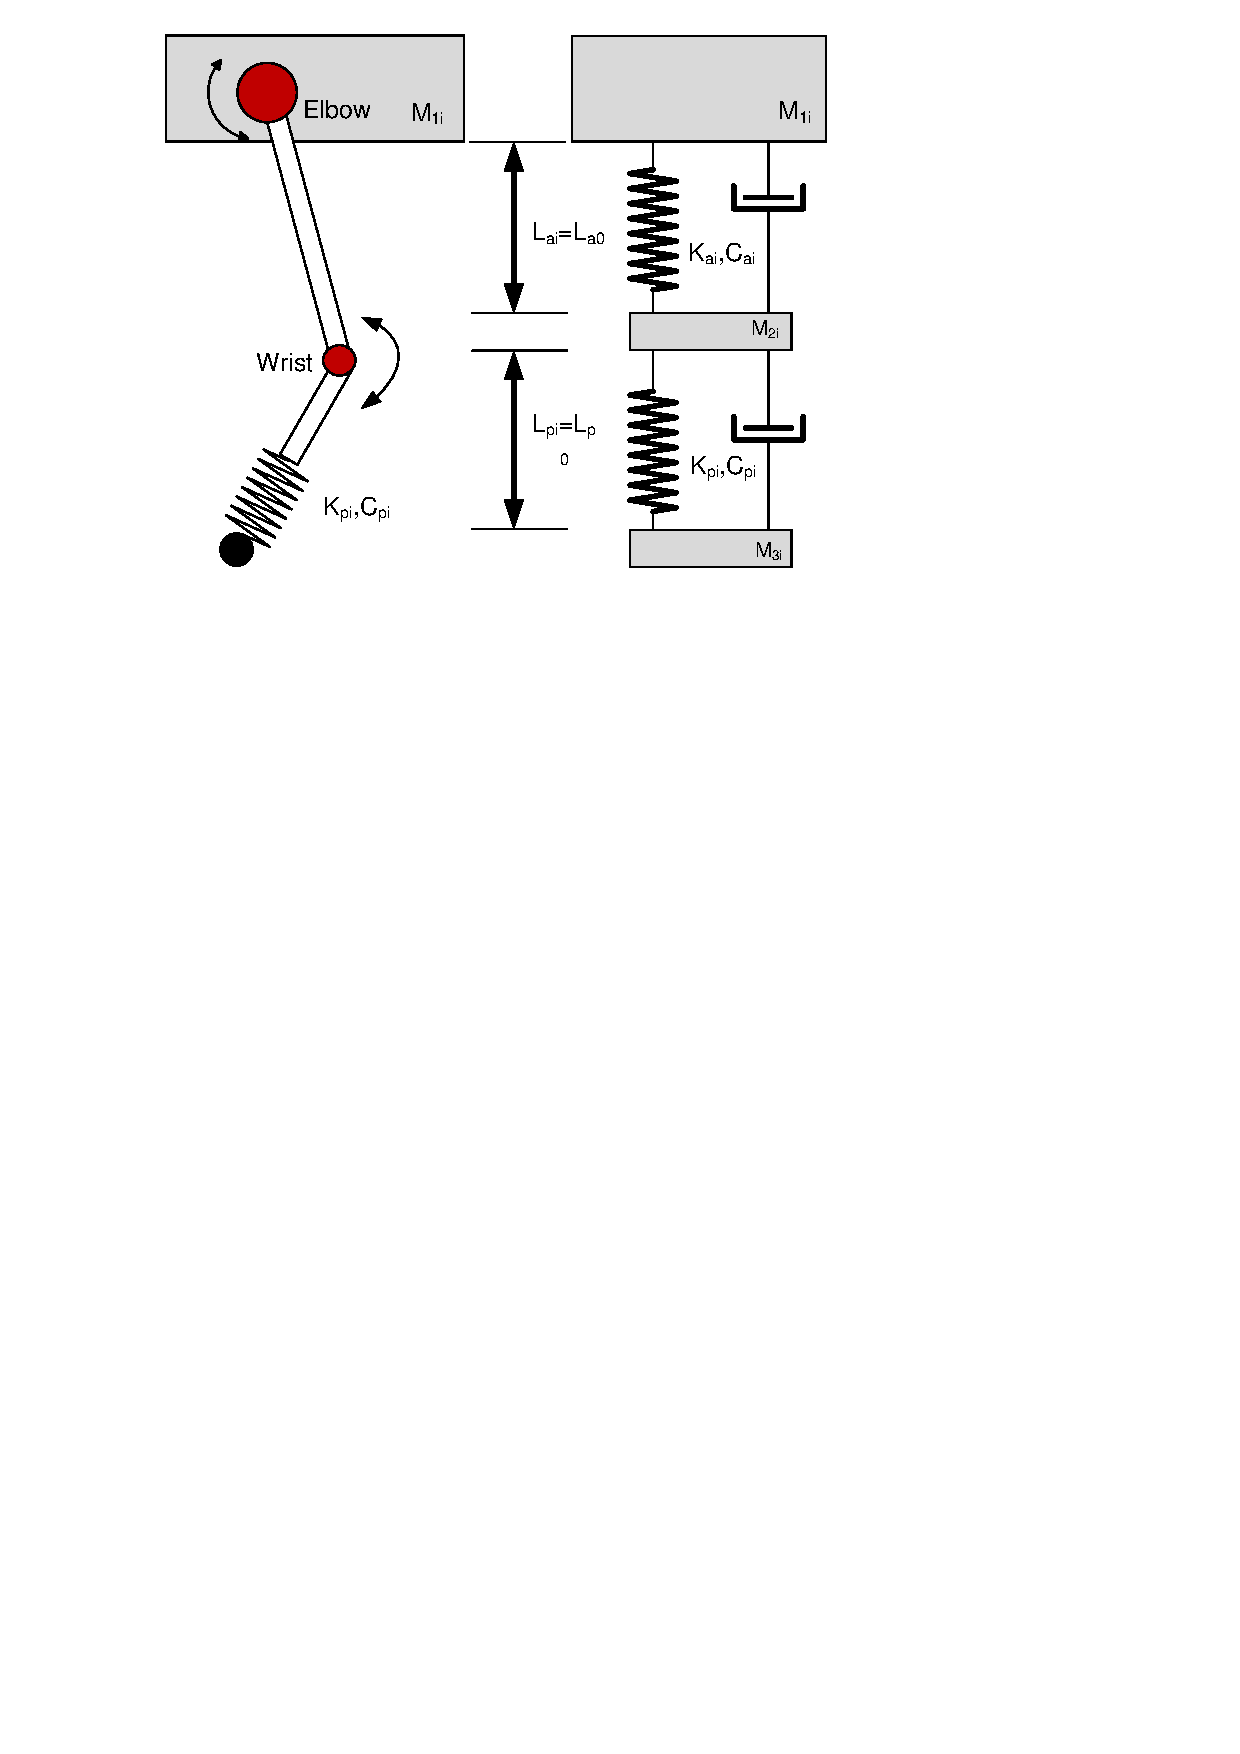
\includegraphics[width=75mm]{./pictures/Dynarobin_leg.pdf}
	\caption{Dynarobin leg model}
	\label{fig:DynarobinLEG}
\end{figure}
